\documentclass[a4paper,13pt]{report}
\usepackage{hyperref}
\usepackage{xcolor} % For colors
\usepackage{fancyhdr}
\usepackage{geometry}
\geometry{margin=1in}
\renewcommand*\thesection{\arabic{section}}
\definecolor{myBlue}{HTML}{6D351A}
\usepackage[explicit]{titlesec}
\usepackage{lmodern}
\usepackage{lipsum}
\usepackage{multirow}
\usepackage{biblatex} 
\usepackage{tabularx}
\usepackage{ctable}
\usepackage{colortbl}
\usepackage{amssymb}
\usepackage{mathtools}
\usepackage{tcolorbox}
\newcolumntype{C}{>{\raggedleft\arraybackslash}X}
\newcommand{\autodot}{\ifnum\value{section}>0.\fi}
 % For custom section formatting
% Custom commands for easy updating
\newcommand{\Title}{Data analysis and Machine Learning}
\newcommand{\Subtitle}{The Institute of Mathematical Sciences}
\newcommand{\Author}{Bhabani Sankar Tripathy}
\newcommand{\Department}{Department of Theoretical Physics}
%\newcommand{\Address}{Wilberforce Road, Cambridge, CB3 OWA, UK}
%\newcommand{\Website}{http://www.damtp.cam.ac.uk/user/tong/qft.html}
\newcommand{\Email}{tbhabanisankar@gmail.com}
\definecolor{auburn}{rgb}{0.43, 0.21, 0.1}
\newtcolorbox[auto counter, number within=section]{note}[2][]{colback=yellow!10!white, colframe=red!50!black, 
	title={Note \thetcbcounter: #2},arc=4mm, fonttitle=\bfseries, #1}



\titleformat{\chapter}[block]{\huge\bfseries\sffamily}%
{}%
{0pt}%
{%
	\begin{tabularx}{\textwidth}{lC}
		\multirow{-2.5}{*}{\fontsize{30}{30}\selectfont\thechapter} & #1\\\arrayrulecolor{red!50!black}\cmidrule[4pt]{2-2}
	\end{tabularx}
}
% Custom section formatting
\titleformat{\section}[block]{\Large\bfseries\sffamily}%
{}%
{0pt}%
{%
	\renewcommand{\arraystretch}{1.5}
	\begin{tabularx}{\textwidth}{p{60pt}X}
		\centering\cellcolor{blue!25} \thechapter.\thesection & #1\\
		\arrayrulecolor{blue!25}\specialrule{.25em}{-0.1em}{0em}
	\end{tabularx}
}
\titlespacing*{\section}{0pt}{3mm}{5mm}
% Header and footer setup
\fancyhf{}
\fancyfoot[C]{\thepage}

% Configure hyperref to hide link borders
\hypersetup{
	colorlinks=true,       % False: boxed links; true: colored links
	linkcolor=black,       % Color of internal links
	citecolor=blue,        % Color of citations
	filecolor=magenta,     % Color of file links
	urlcolor=blue,         % Color of external links
	pdfpagemode=UseNone,   % Do not display bookmarks
	pdfstartview=FitH,     % Fit to width of page
	hidelinks              % Hide links borders
}
% Custom section formatting

\begin{document}
	
	% Title
	\begin{flushleft}
		\vspace*{6.0cm} % Adjust this value to start from the middle
		\textcolor{black}{\textbf{\LARGE \Title}}\\
		\vspace{0.5cm}
		\textcolor{darkgray}{\textbf{\Subtitle}}\\
		\vspace{0.5cm}
		\rule{\textwidth}{1.4pt} % Single horizontal line
	\end{flushleft}
	
	% Author details
	\vspace{0.5cm} % Adjust this value for the vertical space between the line and author details
	\begin{flushleft}
		\textcolor{black}{\large{\textbf{\Author}}}\\
		\textcolor{auburn}{\Department,}\\
		%\Centre,\\
		%\Address\\
		\vspace{0.5cm}
		%\href{\Website}{\Website}\\
		\textcolor{auburn}{\href{mailto:\Email}{\Email}}
	\end{flushleft}
	\newpage

\tableofcontents
\chapter{Recap of Statistics}
\chapter{Probability Distributions, Simple Plots, and Expectation Values} 
The concept that we need to understand is a histogram. A histogram is just a sum of the number of data points that fall within a specific range of x, called a "bin." We can compute it using the \textbf{np.histogram} function. This outputs an array with the number of data points per bin along with the edges of the bin. \\

To fill this histogram, we will generate a set of random values (or events). We will use the \textbf{np.random.uniform} function, which generates random numbers from a uniform distribution. Alternatively we can use \textbf{np.random.normal} to sample our variable with gaussian/normal distribution.\\
\begin{note}[label=mylabel]{Gnerating Random Number}
It's impossible for any computer program to generate truly random numbers. Describing how such generators work in beyond the scope of this course but most programs use a number called the "seed". Using the same starting value for the seed always produces the same set of "random" numbers. 

This seems counterintuitive to the very concept of "random" numbers. However, it is often desirable to have a way to recreate a specific set of random numbers so that a program using sampling can give reproducible results. This is done by setting the starting value of the random seed. 

The point is that, given \textbf{only} the set of generated random numbers, it is not possible to find a pattern that can be used to predict any of the entries given the previous values. The need to generate a reproducible sequence of numbers which, nonetheless, displays no discernible pattern is why random number generators are not trivial to write.
\end{note}
\begin{verbatim}
	bkg = np.random.uniform(0,10, 1000) 
	histy, bin_edges = np.histogram(bkg, bins=20)
	bin_centers = 0.5*(bin_edges[1:] + bin_edges[:-1])
	
	
	#plotting-------------------
	#plot size
	#fig, ax = plt.subplots(figsize=(9,6)) #optionally set the figure size here
	
	#plot data and axes limits
	plt.plot(bin_centers,histy,drawstyle = 'steps-mid',color="r")
\end{verbatim}
           \begin{figure}[h!]
           	\centering
           	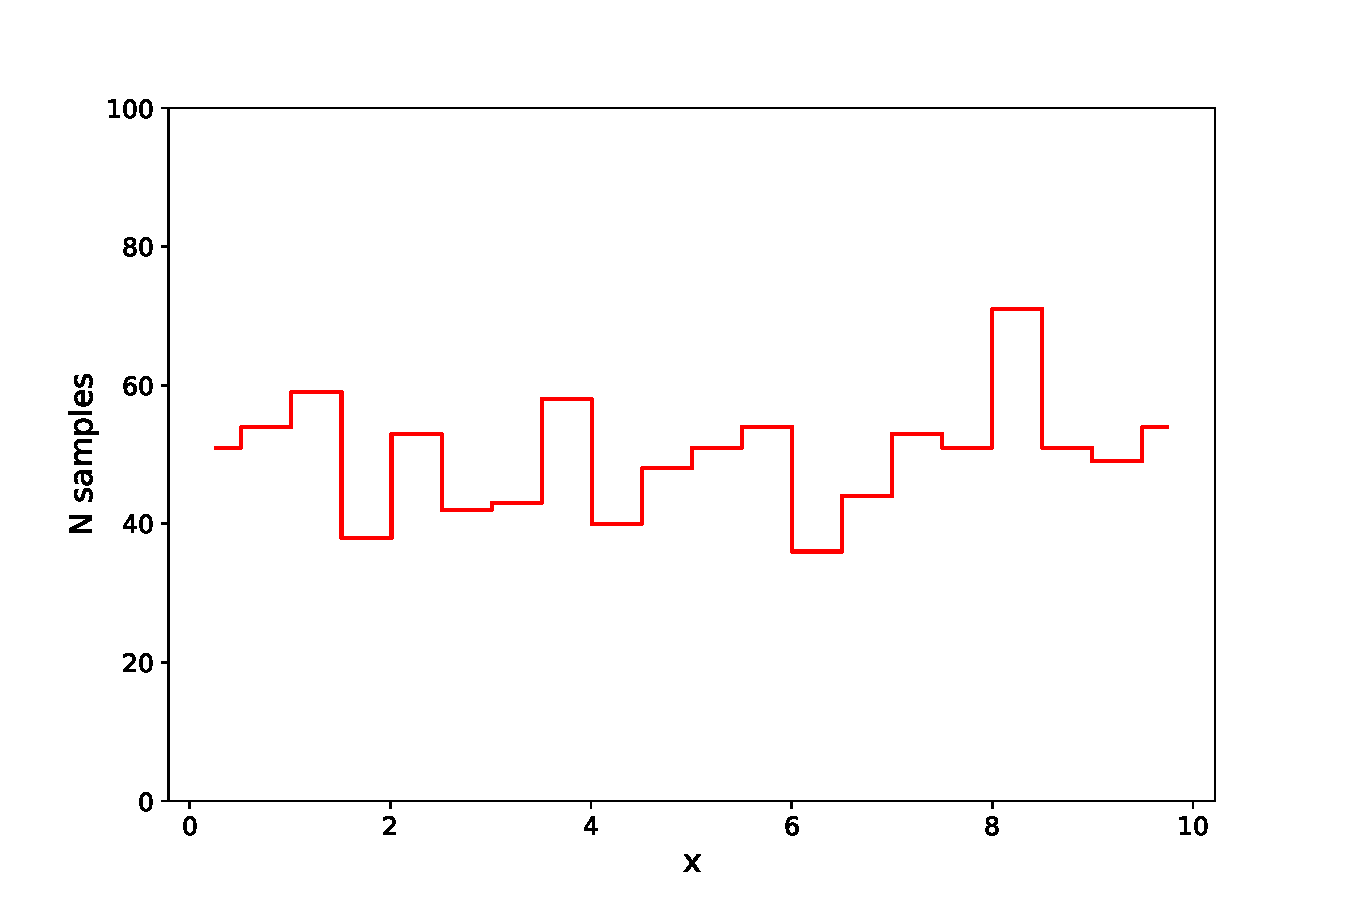
\includegraphics[width=0.8\textwidth]{../lec1pic1.pdf}
           	\label{l1p1}
           	\caption{Histogram of 1000 uniform sample from 0 to 10 with binsize 20}
           \end{figure} 
 What is the integral of the histogram its basically the total sample size here it is 1000.\\
 
 Now lets ask one thing, how the result depends on the number of binsize that we choosed. We plotted the histogram using binsize =3,10,1000 and depicted in fig \ref{l1p2}. For 3 bins we have less idea regarding the distribution as it just divided to its mean value. for 1000 bins we do not have any idea regarding the distribution so it is not a good idea to use very less or very high bin size. It is advisable to use less bin but not close to zero. Its even better to vary our bin size and check the correct one.\\
  \begin{figure}[h!]
 	\centering
 	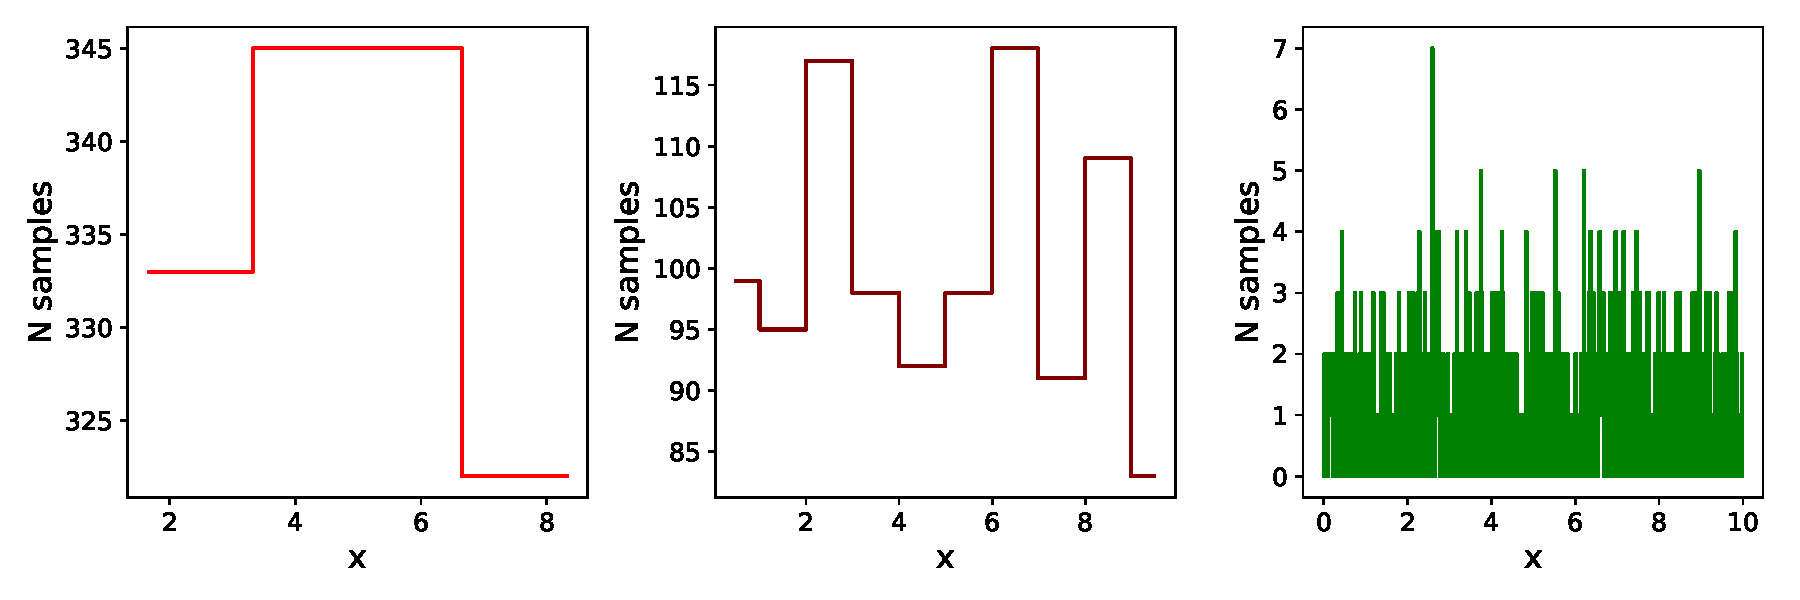
\includegraphics[width=0.8\textwidth]{../lec1pic2.pdf}
 	\label{l1p2}
 	\caption{comparision of Histogram of 1000 uniform sample from 0 to 10 with varying binsize 3,10,1000 from left to right respectively}
 \end{figure}
Let's try something a bit more complicated. In the following code, we are going to sample TWO random variables described by uniform (flat) distributions. Then, we'll define a new random variable that's the SUM of the two sampled values. The "observed" value of a random number (i.e., what you get when you sample a distribution) is also called a ``realization".
\begin{verbatim}
	def getHist(data):
	"""Get hist y values, bin edges, and bin centers as np arrays"""
	histy, bin_edges = np.histogram(data, bins=100)
	bin_centers = 0.5*(bin_edges[1:] + bin_edges[:-1])
	return (histy, bin_edges, bin_centers)
	
	def plotData(data):
	#plotting-------------------
	#plot size
	#fig, ax = plt.subplots(figsize=(9,6)) #optionally set the figure size here
	
	#plot data
	ax1 = plt.gcf().add_subplot(121)
	ax2 = plt.gcf().add_subplot(122)
	histy, bin_edges, bin_centers = getHist(data)
	integral = len(data)
	norm_histy = histy / integral
	ax1.plot(bin_centers,histy,drawstyle = 'steps-mid',color="r")
	ax2.plot(bin_centers,norm_histy,drawstyle = 'steps-mid',color="g")
	#plot labels and style
	ax1.set_xlabel('x', fontsize=15) #Label x
	ax2.set_xlabel('x', fontsize=15)
	ax1.set_ylabel('N samples', fontsize=15) #Label y
	ax2.set_ylabel('Relative probability', fontsize=15)
\end{verbatim}
Now we will plot them individually for flat distributon and normal distribution
\begin{verbatim}
	plotData(data1)
\end{verbatim}
 \begin{figure}[h!]
	\centering
	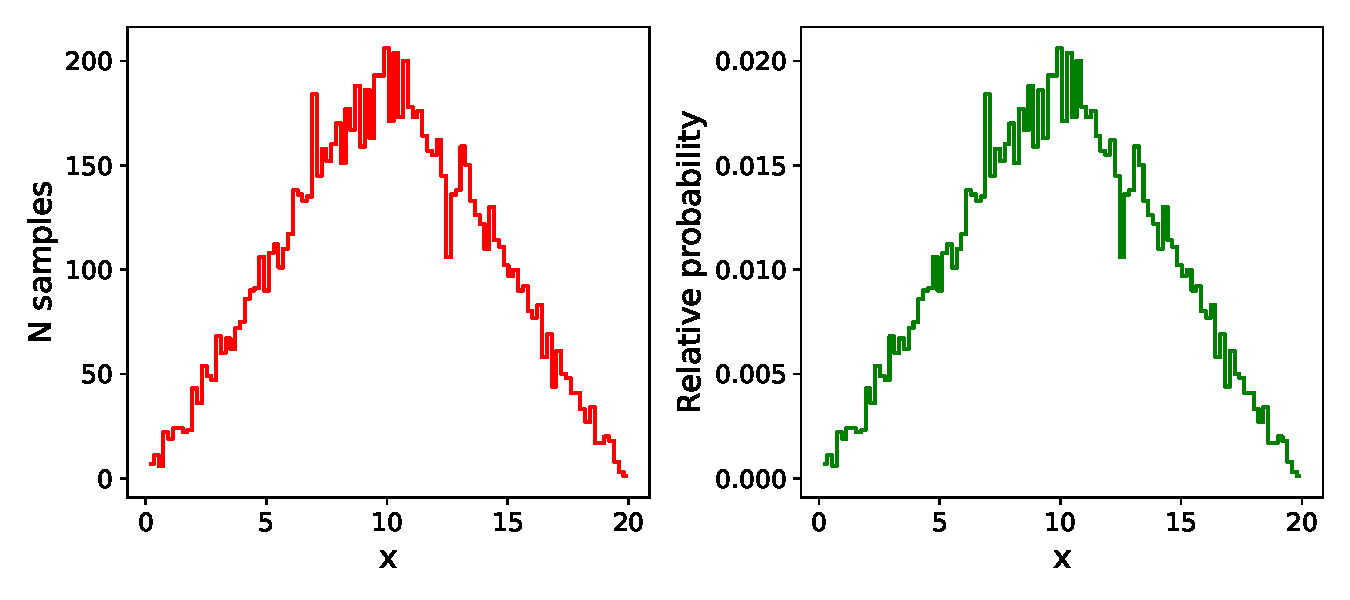
\includegraphics[width=0.8\textwidth]{../lec1pic3.pdf}
	\label{l1p3}
	\caption{comparision of Histogram of 2 10000 uniform sample from 0 to 10 with binsize 100 for uniform distribution}
\end{figure}
\begin{verbatim}
	plotData(data2)
\end{verbatim}
\begin{figure}[h!]
	\centering
	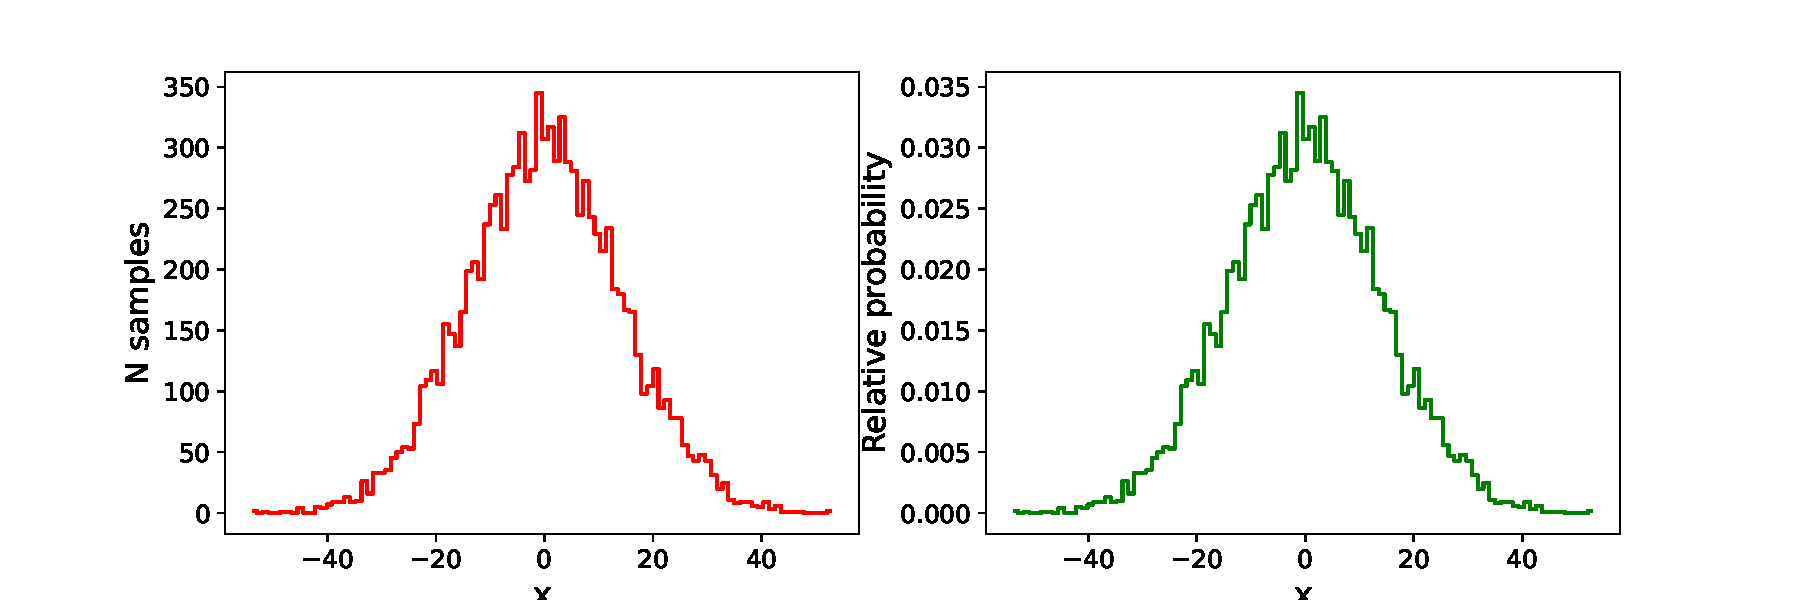
\includegraphics[width=0.8\textwidth]{../lec1pic4.pdf}
	\label{l1p4}
	\caption{comparision of Histogram of 2 10000 uniform sample from 0 to 10 with binsize 100 for normal distribution}
\end{figure}
One of the interesting thing which we can observe is even if we use flat distribution for two variables and when we add them it looks like normal distribution and we will see later that if we use more more such variable it will be close to a gaussian as an application of central limit theorem.\\
So, what distribution are we sampling when we generate this new random variable? \\

Let's derive it analytically. However, before we do that, let's first define a few statistical quantities. When these quantities are calculated for a specific sample of events, they are called ``observables". \\

To understand this, we need to define a probability distribution function, or "PDF". By definition, the integral of a PDF is always equal to 1. \\

When we sample a uniform distribution from 0 to 10, we are sampling random numbers in that range. We can characterize the process of taking a random sample of a PDF $p(x)$ by defining the probability $P_{ab}(X)$ that a number is sampled between $a$ and $b$ as: 

$$P_{ab}(X)=\int_{a}^{b}p(x)dx$$

or, in other words, the probability is given by the integral of $p(x)$ over that range. As expected, the probability of observing a number within the entire range of the PDF will always equal 1. 

$$1=\int_{-\infty}^{\infty}p(x)dx$$

For a flat distribution from a to b, $p(x)$ is given by:

$$p_{flat}(x)=\frac{1}{b-a}$$  

To check this, let's just count events in our range. If we restrict our range to $x_{min} < x < x_{max}$ (where $x_{min} > a$ and $x_{max} < b$), the probability will then be 

$$\int_{x_{min}}^{x_{max}}\frac{1}{b-a}dx = \frac{x_{max}-x_{min}}{b-a}$$
Lets take an example
\begin{verbatim}
	
\end{verbatim}
\section{Binomial Distribution}
Often we perform measurements having some probability. Let's say we perform many equal-probability measurements. What will be our distribution? Since this is not a math class, we will not go into the depth of the math behind this, but let's at least walk through a basic derivation.\\

Let's say you flip a coin 10 times, and the probability of heads is $p$. Let's say you get heads 3 times and tails 7 times.\\

$\bullet$ What are the number of different cases where there are 3 heads?\\

In this case, all we care about is the number of heads out of the total number of flips, so we can use the formula for a \textbf{combination}: $\binom{10}{3}=\frac{10!}{3!(10-3)!}=120$ . As a brief reminder of how this works, there is a total of $10!$ different ordered combinations of our distinct flips 1 through 10. Let's say we identify 3 of those 10 flips as special for whatever reason (e.g. let's take the first 3 flips). Then there are $3!$ ways to order those flips (e.g. (1,2,3),(1,3,2),....) and there are $7!$ ways to order the remaining 7 flips. To find the ``distinct" number of ways a group of 3 and a group of 7 can happen, we divide the total number of different ordered combinations $10!$ by these two groups. Thus, for all 10 flips, there are $\binom{10}{3}$ different ways to order a group of 3 flips and a group of 7 flips, where the group of 3 and the group of 7 are ``distinct" from one another (one example being 1,2,3 is heads and 4...10 is tails). More generally, for $n$ total flips and $m$ heads/tails, the total number of distinct combinations is written as $\frac{n!}{m!(n-m)!}$. \\

\begin{itemize}
 

	\item What is the probability of the scenario where we get 3 heads out of 10 total flips?

	\item Each flip of the coin has equal probability of landing on heads. Let's say that this probability is $p$. With one heads and one tails in two flips, the probability would be the probability to get heads ($p$) multiplied by the probability to get tails ($1-p$), multiplied by the number of distinct combinations that would give you one head and one tail. In this case, the number of combinations is $2$ (heads first and tails second, *or* tails first and heads second). This yields a total probability of $p(1-p)\times N_\mathrm{combo}=2p(1-p)$.

	\item In the case of 10 flips where there are 3 heads, the probability becomes the probability of 3 heads $p^{3}$ multiplied by the probability of 7 tails $(1-p)^{7}$ multiplied by $N_\mathrm{combo}$. In general, for $n$ flips and $m$ heads, we have $p^{m}(1-p)^{n}\times N_\mathrm{combo}$. 



	\item What is the distribution?
	\item If we combine everything for our specific case, we have $_{10}C_{3}\times p^3(1-p)^7$ 
	\item The general formula is actually called the binomial distribution! It is given by $f(m)=p^{m}(1-p)^{n}\frac{n!}{m!(n-m)!}$
\end{itemize}
Let's actually compute this for a few cases!
\end{document}
